\documentclass[1p]{elsarticle_modified}
%\bibliographystyle{elsarticle-num}

%\usepackage[colorlinks]{hyperref}
%\usepackage{abbrmath_seonhwa} %\Abb, \Ascr, \Acal ,\Abf, \Afrak
\usepackage{amsfonts}
\usepackage{amssymb}
\usepackage{amsmath}
\usepackage{amsthm}
\usepackage{scalefnt}
\usepackage{amsbsy}
\usepackage{kotex}
\usepackage{caption}
\usepackage{subfig}
\usepackage{color}
\usepackage{graphicx}
\usepackage{xcolor} %% white, black, red, green, blue, cyan, magenta, yellow
\usepackage{float}
\usepackage{setspace}
\usepackage{hyperref}

\usepackage{tikz}
\usetikzlibrary{arrows}

\usepackage{multirow}
\usepackage{array} % fixed length table
\usepackage{hhline}

%%%%%%%%%%%%%%%%%%%%%
\makeatletter
\renewcommand*\env@matrix[1][\arraystretch]{%
	\edef\arraystretch{#1}%
	\hskip -\arraycolsep
	\let\@ifnextchar\new@ifnextchar
	\array{*\c@MaxMatrixCols c}}
\makeatother %https://tex.stackexchange.com/questions/14071/how-can-i-increase-the-line-spacing-in-a-matrix
%%%%%%%%%%%%%%%

\usepackage[normalem]{ulem}

\newcommand{\msout}[1]{\ifmmode\text{\sout{\ensuremath{#1}}}\else\sout{#1}\fi}
%SOURCE: \msout is \stkout macro in https://tex.stackexchange.com/questions/20609/strikeout-in-math-mode

\newcommand{\cancel}[1]{
	\ifmmode
	{\color{red}\msout{#1}}
	\else
	{\color{red}\sout{#1}}
	\fi
}

\newcommand{\add}[1]{
	{\color{blue}\uwave{#1}}
}

\newcommand{\replace}[2]{
	\ifmmode
	{\color{red}\msout{#1}}{\color{blue}\uwave{#2}}
	\else
	{\color{red}\sout{#1}}{\color{blue}\uwave{#2}}
	\fi
}

\newcommand{\Sol}{\mathcal{S}} %segment
\newcommand{\D}{D} %diagram
\newcommand{\A}{\mathcal{A}} %arc


%%%%%%%%%%%%%%%%%%%%%%%%%%%%%5 test

\def\sl{\operatorname{\textup{SL}}(2,\Cbb)}
\def\psl{\operatorname{\textup{PSL}}(2,\Cbb)}
\def\quan{\mkern 1mu \triangleright \mkern 1mu}

\theoremstyle{definition}
\newtheorem{thm}{Theorem}[section]
\newtheorem{prop}[thm]{Proposition}
\newtheorem{lem}[thm]{Lemma}
\newtheorem{ques}[thm]{Question}
\newtheorem{cor}[thm]{Corollary}
\newtheorem{defn}[thm]{Definition}
\newtheorem{exam}[thm]{Example}
\newtheorem{rmk}[thm]{Remark}
\newtheorem{alg}[thm]{Algorithm}

\newcommand{\I}{\sqrt{-1}}
\begin{document}

%\begin{frontmatter}
%
%\title{Boundary parabolic representations of knots up to 8 crossings}
%
%%% Group authors per affiliation:
%\author{Yunhi Cho} 
%\address{Department of Mathematics, University of Seoul, Seoul, Korea}
%\ead{yhcho@uos.ac.kr}
%
%
%\author{Seonhwa Kim} %\fnref{s_kim}}
%\address{Center for Geometry and Physics, Institute for Basic Science, Pohang, 37673, Korea}
%\ead{ryeona17@ibs.re.kr}
%
%\author{Hyuk Kim}
%\address{Department of Mathematical Sciences, Seoul National University, Seoul 08826, Korea}
%\ead{hyukkim@snu.ac.kr}
%
%\author{Seokbeom Yoon}
%\address{Department of Mathematical Sciences, Seoul National University, Seoul, 08826,  Korea}
%\ead{sbyoon15@snu.ac.kr}
%
%\begin{abstract}
%We find all boundary parabolic representation of knots up to 8 crossings.
%
%\end{abstract}
%\begin{keyword}
%    \MSC[2010] 57M25 
%\end{keyword}
%
%\end{frontmatter}

%\linenumbers
%\tableofcontents
%
\newcommand\colored[1]{\textcolor{white}{\rule[-0.35ex]{0.8em}{1.4ex}}\kern-0.8em\color{red} #1}%
%\newcommand\colored[1]{\textcolor{white}{ #1}\kern-2.17ex	\textcolor{white}{ #1}\kern-1.81ex	\textcolor{white}{ #1}\kern-2.15ex\color{red}#1	}

{\Large $\underline{11a_{197}~(K11a_{197})}$}

\setlength{\tabcolsep}{10pt}
\renewcommand{\arraystretch}{1.6}
\vspace{1cm}\begin{tabular}{m{100pt}>{\centering\arraybackslash}m{274pt}}
\multirow{5}{120pt}{
	\centering
	\includegraphics[width=112pt]{../../../GIT/diagram.site/Diagrams/png/446_11a_197.png}\\
\ \ \ A knot diagram\footnotemark}&
\allowdisplaybreaks
\textbf{Linearized knot diagam} \\
\cline{2-2}
 &
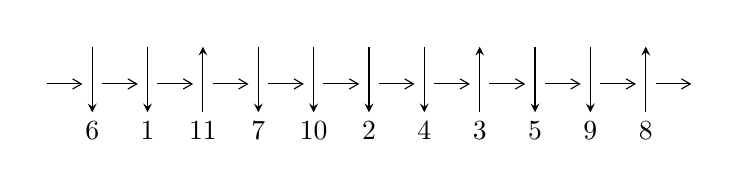
\begin{tikzpicture}[x=20pt, y=17pt]
	% nodes
	\node (C0) at (0, 0) {};
	\node (C1) at (1, 0) {};
	\node (C1U) at (1, +1) {};
	\node (C1D) at (1, -1) {6};

	\node (C2) at (2, 0) {};
	\node (C2U) at (2, +1) {};
	\node (C2D) at (2, -1) {1};

	\node (C3) at (3, 0) {};
	\node (C3U) at (3, +1) {};
	\node (C3D) at (3, -1) {11};

	\node (C4) at (4, 0) {};
	\node (C4U) at (4, +1) {};
	\node (C4D) at (4, -1) {7};

	\node (C5) at (5, 0) {};
	\node (C5U) at (5, +1) {};
	\node (C5D) at (5, -1) {10};

	\node (C6) at (6, 0) {};
	\node (C6U) at (6, +1) {};
	\node (C6D) at (6, -1) {2};

	\node (C7) at (7, 0) {};
	\node (C7U) at (7, +1) {};
	\node (C7D) at (7, -1) {4};

	\node (C8) at (8, 0) {};
	\node (C8U) at (8, +1) {};
	\node (C8D) at (8, -1) {3};

	\node (C9) at (9, 0) {};
	\node (C9U) at (9, +1) {};
	\node (C9D) at (9, -1) {5};

	\node (C10) at (10, 0) {};
	\node (C10U) at (10, +1) {};
	\node (C10D) at (10, -1) {9};

	\node (C11) at (11, 0) {};
	\node (C11U) at (11, +1) {};
	\node (C11D) at (11, -1) {8};
	\node (C12) at (12, 0) {};

	% arrows
	\draw[->,>={angle 60}]
	(C0) edge (C1) (C1) edge (C2) (C2) edge (C3) (C3) edge (C4) (C4) edge (C5) (C5) edge (C6) (C6) edge (C7) (C7) edge (C8) (C8) edge (C9) (C9) edge (C10) (C10) edge (C11) (C11) edge (C12) ;	\draw[->,>=stealth]
	(C1U) edge (C1D) (C2U) edge (C2D) (C3D) edge (C3U) (C4U) edge (C4D) (C5U) edge (C5D) (C6U) edge (C6D) (C7U) edge (C7D) (C8D) edge (C8U) (C9U) edge (C9D) (C10U) edge (C10D) (C11D) edge (C11U) ;
	\end{tikzpicture} \\
\hhline{~~} \\& 
\textbf{Solving Sequence} \\ \cline{2-2} 
 &
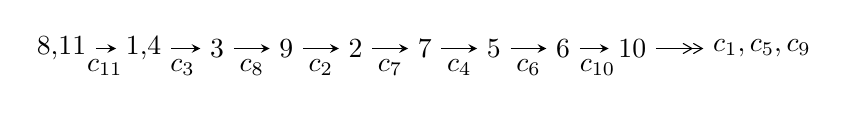
\begin{tikzpicture}[x=25pt, y=7pt]
	% node
	\node (A0) at (-1/8, 0) {8,11};
	\node (A1) at (17/16, 0) {1,4};
	\node (A2) at (17/8, 0) {3};
	\node (A3) at (25/8, 0) {9};
	\node (A4) at (33/8, 0) {2};
	\node (A5) at (41/8, 0) {7};
	\node (A6) at (49/8, 0) {5};
	\node (A7) at (57/8, 0) {6};
	\node (A8) at (65/8, 0) {10};
	\node (C1) at (1/2, -1) {$c_{11}$};
	\node (C2) at (13/8, -1) {$c_{3}$};
	\node (C3) at (21/8, -1) {$c_{8}$};
	\node (C4) at (29/8, -1) {$c_{2}$};
	\node (C5) at (37/8, -1) {$c_{7}$};
	\node (C6) at (45/8, -1) {$c_{4}$};
	\node (C7) at (53/8, -1) {$c_{6}$};
	\node (C8) at (61/8, -1) {$c_{10}$};
	\node (A9) at (10, 0) {$c_{1},c_{5},c_{9}$};

	% edge
	\draw[->,>=stealth]	
	(A0) edge (A1) (A1) edge (A2) (A2) edge (A3) (A3) edge (A4) (A4) edge (A5) (A5) edge (A6) (A6) edge (A7) (A7) edge (A8) ;
	\draw[->>,>={angle 60}]	
	(A8) edge (A9);
\end{tikzpicture} \\ 

\end{tabular} \\

\footnotetext{
The image of knot diagram is generated by the software ``\textbf{Draw programme}" developed by Andrew Bartholomew(\url{http://www.layer8.co.uk/maths/draw/index.htm\#Running-draw}), where we modified some parts for our purpose(\url{https://github.com/CATsTAILs/LinksPainter}).
}\phantom \\ \newline 
\centering \textbf{Ideals for irreducible components\footnotemark of $X_{\text{par}}$} 
 
\begin{align*}
I^u_{1}&=\langle 
b- u,\;1133732 u^{18}-5530440 u^{17}+\cdots+1639243 a+14603996,\;u^{19}-3 u^{17}+\cdots+5 u+1\rangle \\
I^u_{2}&=\langle 
4.04940\times10^{223} u^{67}+3.30886\times10^{224} u^{66}+\cdots+4.64646\times10^{224} b-5.28089\times10^{226},\\
\phantom{I^u_{2}}&\phantom{= \langle  }2.91872\times10^{228} u^{67}+2.08756\times10^{229} u^{66}+\cdots+5.97071\times10^{227} a-5.77931\times10^{230},\\
\phantom{I^u_{2}}&\phantom{= \langle  }u^{68}+7 u^{67}+\cdots+375 u+257\rangle \\
I^u_{3}&=\langle 
b+u,\;u^7+u^6-2 u^4+u^2+a+2 u-1,\;u^8- u^6- u^5+2 u^4- u+1\rangle \\
I^u_{4}&=\langle 
-3 u^7-2 u^6+2 u^5-4 u^4+3 u^2+b-7 u+4,\;-4 u^7-3 u^6+2 u^5-6 u^4- u^3+3 u^2+a-9 u+5,\\
\phantom{I^u_{4}}&\phantom{= \langle  }u^8- u^6+2 u^5- u^4- u^3+3 u^2-3 u+1\rangle \\
\\
\end{align*}
\raggedright * 4 irreducible components of $\dim_{\mathbb{C}}=0$, with total 103 representations.\\
\footnotetext{All coefficients of polynomials are rational numbers. But the coefficients are sometimes approximated in decimal forms when there is not enough margin.}
\newpage
\renewcommand{\arraystretch}{1}
\centering \section*{I. $I^u_{1}= \langle b- u,\;1.13\times10^{6} u^{18}-5.53\times10^{6} u^{17}+\cdots+1.64\times10^{6} a+1.46\times10^{7},\;u^{19}-3 u^{17}+\cdots+5 u+1 \rangle$}
\flushleft \textbf{(i) Arc colorings}\\
\begin{tabular}{m{7pt} m{180pt} m{7pt} m{180pt} }
\flushright $a_{8}=$&$\begin{pmatrix}0\\u\end{pmatrix}$ \\
\flushright $a_{11}=$&$\begin{pmatrix}1\\0\end{pmatrix}$ \\
\flushright $a_{1}=$&$\begin{pmatrix}1\\- u^2\end{pmatrix}$ \\
\flushright $a_{4}=$&$\begin{pmatrix}-0.691619 u^{18}+3.37378 u^{17}+\cdots-28.3695 u-8.90899\\u\end{pmatrix}$ \\
\flushright $a_{3}=$&$\begin{pmatrix}-0.691619 u^{18}+3.37378 u^{17}+\cdots-29.3695 u-8.90899\\u\end{pmatrix}$ \\
\flushright $a_{9}=$&$\begin{pmatrix}-4.15807 u^{18}-6.66141 u^{17}+\cdots+52.3548 u+8.42543\\0.622113 u^{18}+1.86560 u^{17}+\cdots-15.1773 u-3.37378\end{pmatrix}$ \\
\flushright $a_{2}=$&$\begin{pmatrix}-0.0695059 u^{18}+5.23938 u^{17}+\cdots-44.5467 u-12.2828\\-0.756830 u^{18}-1.16457 u^{17}+\cdots+10.9501 u+1.86560\end{pmatrix}$ \\
\flushright $a_{7}=$&$\begin{pmatrix}-2.91384 u^{18}-2.93021 u^{17}+\cdots+20.0003 u+1.67787\\0.622113 u^{18}+1.86560 u^{17}+\cdots-15.1773 u-3.37378\end{pmatrix}$ \\
\flushright $a_{5}=$&$\begin{pmatrix}4.05196 u^{18}-2.08218 u^{17}+\cdots+21.9378 u+3.05750\\-1.38107 u^{18}-0.495631 u^{17}+\cdots+2.38762 u-0.443568\end{pmatrix}$ \\
\flushright $a_{6}=$&$\begin{pmatrix}4.07319 u^{18}+0.0169841 u^{17}+\cdots-3.37920 u-2.08628\\-1.50818 u^{18}+0.134717 u^{17}+\cdots-1.03345 u-1.31373\end{pmatrix}$ \\
\flushright $a_{10}=$&$\begin{pmatrix}1.53997 u^{18}-5.15071 u^{17}+\cdots+38.3233 u+9.86555\\0.959164 u^{18}+1.36657 u^{17}+\cdots-11.2769 u-2.27262\end{pmatrix}$\\ \flushright $a_{10}=$&$\begin{pmatrix}1.53997 u^{18}-5.15071 u^{17}+\cdots+38.3233 u+9.86555\\0.959164 u^{18}+1.36657 u^{17}+\cdots-11.2769 u-2.27262\end{pmatrix}$\\&\end{tabular}
\flushleft \textbf{(ii) Obstruction class $= -1$}\\~\\
\flushleft \textbf{(iii) Cusp Shapes $= -\frac{18167001}{1639243} u^{18}-\frac{11571693}{1639243} u^{17}+\cdots+\frac{103230908}{1639243} u-\frac{4877099}{1639243}$}\\~\\
\newpage\renewcommand{\arraystretch}{1}
\flushleft \textbf{(iv) u-Polynomials at the component}\newline \\
\begin{tabular}{m{50pt}|m{274pt}}
Crossings & \hspace{64pt}u-Polynomials at each crossing \\
\hline $$\begin{aligned}c_{1},c_{5},c_{6}\\c_{9}\end{aligned}$$&$\begin{aligned}
&u^{19}-4 u^{17}+\cdots- u+1
\end{aligned}$\\
\hline $$\begin{aligned}c_{2},c_{10}\end{aligned}$$&$\begin{aligned}
&u^{19}+8 u^{18}+\cdots+5 u+1
\end{aligned}$\\
\hline $$\begin{aligned}c_{3},c_{11}\end{aligned}$$&$\begin{aligned}
&u^{19}-3 u^{17}+\cdots+5 u+1
\end{aligned}$\\
\hline $$\begin{aligned}c_{4},c_{7}\end{aligned}$$&$\begin{aligned}
&u^{19}-12 u^{18}+\cdots-224 u+32
\end{aligned}$\\
\hline $$\begin{aligned}c_{8}\end{aligned}$$&$\begin{aligned}
&u^{19}-18 u^{18}+\cdots-1184 u+192
\end{aligned}$\\
\hline
\end{tabular}\\~\\
\newpage\renewcommand{\arraystretch}{1}
\flushleft \textbf{(v) Riley Polynomials at the component}\newline \\
\begin{tabular}{m{50pt}|m{274pt}}
Crossings & \hspace{64pt}Riley Polynomials at each crossing \\
\hline $$\begin{aligned}c_{1},c_{5},c_{6}\\c_{9}\end{aligned}$$&$\begin{aligned}
&y^{19}-8 y^{18}+\cdots+5 y-1
\end{aligned}$\\
\hline $$\begin{aligned}c_{2},c_{10}\end{aligned}$$&$\begin{aligned}
&y^{19}+12 y^{18}+\cdots-23 y-1
\end{aligned}$\\
\hline $$\begin{aligned}c_{3},c_{11}\end{aligned}$$&$\begin{aligned}
&y^{19}-6 y^{18}+\cdots+29 y-1
\end{aligned}$\\
\hline $$\begin{aligned}c_{4},c_{7}\end{aligned}$$&$\begin{aligned}
&y^{19}+12 y^{18}+\cdots+1536 y-1024
\end{aligned}$\\
\hline $$\begin{aligned}c_{8}\end{aligned}$$&$\begin{aligned}
&y^{19}-4 y^{18}+\cdots+50176 y-36864
\end{aligned}$\\
\hline
\end{tabular}\\~\\
\newpage\flushleft \textbf{(vi) Complex Volumes and Cusp Shapes}
$$\begin{array}{c|c|c}  
\text{Solutions to }I^u_{1}& \I (\text{vol} + \sqrt{-1}CS) & \text{Cusp shape}\\
 \hline 
\begin{aligned}
u &= \phantom{-}0.922328 + 0.410149 I \\
a &= -0.097023 + 0.610902 I \\
b &= \phantom{-}0.922328 + 0.410149 I\end{aligned}
 & \phantom{-}1.76273 + 1.04354 I & \phantom{-}2.78842 - 1.15879 I \\ \hline\begin{aligned}
u &= \phantom{-}0.922328 - 0.410149 I \\
a &= -0.097023 - 0.610902 I \\
b &= \phantom{-}0.922328 - 0.410149 I\end{aligned}
 & \phantom{-}1.76273 - 1.04354 I & \phantom{-}2.78842 + 1.15879 I \\ \hline\begin{aligned}
u &= -0.299279 + 0.864422 I \\
a &= \phantom{-}0.725338 + 0.593270 I \\
b &= -0.299279 + 0.864422 I\end{aligned}
 & -5.58807 + 2.35049 I & -13.53566 - 3.60952 I \\ \hline\begin{aligned}
u &= -0.299279 - 0.864422 I \\
a &= \phantom{-}0.725338 - 0.593270 I \\
b &= -0.299279 - 0.864422 I\end{aligned}
 & -5.58807 - 2.35049 I & -13.53566 + 3.60952 I \\ \hline\begin{aligned}
u &= \phantom{-}0.935316 + 0.630010 I \\
a &= -0.525722 + 0.984674 I \\
b &= \phantom{-}0.935316 + 0.630010 I\end{aligned}
 & \phantom{-}2.13851 + 0.27818 I & -1.57258 + 0.84514 I \\ \hline\begin{aligned}
u &= \phantom{-}0.935316 - 0.630010 I \\
a &= -0.525722 - 0.984674 I \\
b &= \phantom{-}0.935316 - 0.630010 I\end{aligned}
 & \phantom{-}2.13851 - 0.27818 I & -1.57258 - 0.84514 I \\ \hline\begin{aligned}
u &= \phantom{-}0.864210 + 0.035102 I \\
a &= -0.89308 + 1.80124 I \\
b &= \phantom{-}0.864210 + 0.035102 I\end{aligned}
 & \phantom{-}4.69963 + 7.70569 I & \phantom{-}1.03497 - 7.90507 I \\ \hline\begin{aligned}
u &= \phantom{-}0.864210 - 0.035102 I \\
a &= -0.89308 - 1.80124 I \\
b &= \phantom{-}0.864210 - 0.035102 I\end{aligned}
 & \phantom{-}4.69963 - 7.70569 I & \phantom{-}1.03497 + 7.90507 I \\ \hline\begin{aligned}
u &= -0.826242 + 0.780318 I \\
a &= \phantom{-}0.848642 + 0.882375 I \\
b &= -0.826242 + 0.780318 I\end{aligned}
 & \phantom{-}0.40114 - 10.64020 I & -4.95980 + 10.11213 I \\ \hline\begin{aligned}
u &= -0.826242 - 0.780318 I \\
a &= \phantom{-}0.848642 - 0.882375 I \\
b &= -0.826242 - 0.780318 I\end{aligned}
 & \phantom{-}0.40114 + 10.64020 I & -4.95980 - 10.11213 I\\
 \hline 
 \end{array}$$\newpage$$\begin{array}{c|c|c}  
\text{Solutions to }I^u_{1}& \I (\text{vol} + \sqrt{-1}CS) & \text{Cusp shape}\\
 \hline 
\begin{aligned}
u &= -0.819203 + 0.976775 I \\
a &= -0.346065 + 0.826042 I \\
b &= -0.819203 + 0.976775 I\end{aligned}
 & -3.89495 - 2.33301 I & -11.16071 + 2.50399 I \\ \hline\begin{aligned}
u &= -0.819203 - 0.976775 I \\
a &= -0.346065 - 0.826042 I \\
b &= -0.819203 - 0.976775 I\end{aligned}
 & -3.89495 + 2.33301 I & -11.16071 - 2.50399 I \\ \hline\begin{aligned}
u &= -0.650261 + 0.049079 I \\
a &= \phantom{-}0.38648 + 2.74023 I \\
b &= -0.650261 + 0.049079 I\end{aligned}
 & \phantom{-}6.12689 + 2.86646 I & \phantom{-}4.56371 - 2.58319 I \\ \hline\begin{aligned}
u &= -0.650261 - 0.049079 I \\
a &= \phantom{-}0.38648 - 2.74023 I \\
b &= -0.650261 - 0.049079 I\end{aligned}
 & \phantom{-}6.12689 - 2.86646 I & \phantom{-}4.56371 + 2.58319 I \\ \hline\begin{aligned}
u &= \phantom{-}1.27254 + 0.88593 I \\
a &= \phantom{-}0.346542 + 0.895806 I \\
b &= \phantom{-}1.27254 + 0.88593 I\end{aligned}
 & \phantom{-}8.44383 + 4.90113 I & \phantom{-}0.70738 - 1.64116 I \\ \hline\begin{aligned}
u &= \phantom{-}1.27254 - 0.88593 I \\
a &= \phantom{-}0.346542 - 0.895806 I \\
b &= \phantom{-}1.27254 - 0.88593 I\end{aligned}
 & \phantom{-}8.44383 - 4.90113 I & \phantom{-}0.70738 + 1.64116 I \\ \hline\begin{aligned}
u &= -1.29108 + 0.99217 I \\
a &= -0.262717 + 0.934110 I \\
b &= -1.29108 + 0.99217 I\end{aligned}
 & \phantom{-}5.2789 - 17.4106 I & -3.33834 + 9.88959 I \\ \hline\begin{aligned}
u &= -1.29108 - 0.99217 I \\
a &= -0.262717 - 0.934110 I \\
b &= -1.29108 - 0.99217 I\end{aligned}
 & \phantom{-}5.2789 + 17.4106 I & -3.33834 - 9.88959 I \\ \hline\begin{aligned}
u &= -0.216670\phantom{ +0.000000I} \\
a &= -2.36478\phantom{ +0.000000I} \\
b &= -0.216670\phantom{ +0.000000I}\end{aligned}
 & -0.903842\phantom{ +0.000000I} & -11.0550\phantom{ +0.000000I}\\
 \hline 
 \end{array}$$\newpage\newpage\renewcommand{\arraystretch}{1}
\centering \section*{II. $I^u_{2}= \langle 4.05\times10^{223} u^{67}+3.31\times10^{224} u^{66}+\cdots+4.65\times10^{224} b-5.28\times10^{226},\;2.92\times10^{228} u^{67}+2.09\times10^{229} u^{66}+\cdots+5.97\times10^{227} a-5.78\times10^{230},\;u^{68}+7 u^{67}+\cdots+375 u+257 \rangle$}
\flushleft \textbf{(i) Arc colorings}\\
\begin{tabular}{m{7pt} m{180pt} m{7pt} m{180pt} }
\flushright $a_{8}=$&$\begin{pmatrix}0\\u\end{pmatrix}$ \\
\flushright $a_{11}=$&$\begin{pmatrix}1\\0\end{pmatrix}$ \\
\flushright $a_{1}=$&$\begin{pmatrix}1\\- u^2\end{pmatrix}$ \\
\flushright $a_{4}=$&$\begin{pmatrix}-4.88839 u^{67}-34.9634 u^{66}+\cdots+4825.34 u+967.944\\-0.0871501 u^{67}-0.712125 u^{66}+\cdots+396.084 u+113.654\end{pmatrix}$ \\
\flushright $a_{3}=$&$\begin{pmatrix}-4.80124 u^{67}-34.2513 u^{66}+\cdots+4429.26 u+854.290\\-0.0871501 u^{67}-0.712125 u^{66}+\cdots+396.084 u+113.654\end{pmatrix}$ \\
\flushright $a_{9}=$&$\begin{pmatrix}-7.99115 u^{67}-60.4866 u^{66}+\cdots+10430.3 u+3443.31\\1.61940 u^{67}+12.4687 u^{66}+\cdots-2290.63 u-756.650\end{pmatrix}$ \\
\flushright $a_{2}=$&$\begin{pmatrix}-6.77651 u^{67}-48.1052 u^{66}+\cdots+6300.23 u+1133.09\\0.666031 u^{67}+4.36174 u^{66}+\cdots-121.691 u+106.711\end{pmatrix}$ \\
\flushright $a_{7}=$&$\begin{pmatrix}-4.48948 u^{67}-33.7015 u^{66}+\cdots+5341.98 u+1665.92\\1.88227 u^{67}+14.3164 u^{66}+\cdots-2795.65 u-1020.74\end{pmatrix}$ \\
\flushright $a_{5}=$&$\begin{pmatrix}1.28662 u^{67}+6.44767 u^{66}+\cdots-34.9011 u+812.874\\0.546402 u^{67}+5.09202 u^{66}+\cdots-1326.15 u-757.561\end{pmatrix}$ \\
\flushright $a_{6}=$&$\begin{pmatrix}-4.16324 u^{67}-34.1080 u^{66}+\cdots+8461.50 u+3399.72\\0.717867 u^{67}+6.15447 u^{66}+\cdots-1764.97 u-755.279\end{pmatrix}$ \\
\flushright $a_{10}=$&$\begin{pmatrix}-5.80661 u^{67}-43.0967 u^{66}+\cdots+4592.48 u+1354.29\\2.28558 u^{67}+17.7608 u^{66}+\cdots-2796.80 u-1065.18\end{pmatrix}$\\ \flushright $a_{10}=$&$\begin{pmatrix}-5.80661 u^{67}-43.0967 u^{66}+\cdots+4592.48 u+1354.29\\2.28558 u^{67}+17.7608 u^{66}+\cdots-2796.80 u-1065.18\end{pmatrix}$\\&\end{tabular}
\flushleft \textbf{(ii) Obstruction class $= -1$}\\~\\
\flushleft \textbf{(iii) Cusp Shapes $= 0.644686 u^{67}+6.72660 u^{66}+\cdots-1138.68 u-1495.39$}\\~\\
\newpage\renewcommand{\arraystretch}{1}
\flushleft \textbf{(iv) u-Polynomials at the component}\newline \\
\begin{tabular}{m{50pt}|m{274pt}}
Crossings & \hspace{64pt}u-Polynomials at each crossing \\
\hline $$\begin{aligned}c_{1},c_{5},c_{6}\\c_{9}\end{aligned}$$&$\begin{aligned}
&u^{68}- u^{67}+\cdots-12 u+1
\end{aligned}$\\
\hline $$\begin{aligned}c_{2},c_{10}\end{aligned}$$&$\begin{aligned}
&u^{68}+25 u^{67}+\cdots+60 u+1
\end{aligned}$\\
\hline $$\begin{aligned}c_{3},c_{11}\end{aligned}$$&$\begin{aligned}
&u^{68}+7 u^{67}+\cdots+375 u+257
\end{aligned}$\\
\hline $$\begin{aligned}c_{4},c_{7}\end{aligned}$$&$\begin{aligned}
&(u^{34}+5 u^{33}+\cdots+34 u+5)^{2}
\end{aligned}$\\
\hline $$\begin{aligned}c_{8}\end{aligned}$$&$\begin{aligned}
&(u^{34}+9 u^{33}+\cdots+4 u+1)^{2}
\end{aligned}$\\
\hline
\end{tabular}\\~\\
\newpage\renewcommand{\arraystretch}{1}
\flushleft \textbf{(v) Riley Polynomials at the component}\newline \\
\begin{tabular}{m{50pt}|m{274pt}}
Crossings & \hspace{64pt}Riley Polynomials at each crossing \\
\hline $$\begin{aligned}c_{1},c_{5},c_{6}\\c_{9}\end{aligned}$$&$\begin{aligned}
&y^{68}-25 y^{67}+\cdots-60 y+1
\end{aligned}$\\
\hline $$\begin{aligned}c_{2},c_{10}\end{aligned}$$&$\begin{aligned}
&y^{68}+39 y^{67}+\cdots-600 y+1
\end{aligned}$\\
\hline $$\begin{aligned}c_{3},c_{11}\end{aligned}$$&$\begin{aligned}
&y^{68}-15 y^{67}+\cdots-2055275 y+66049
\end{aligned}$\\
\hline $$\begin{aligned}c_{4},c_{7}\end{aligned}$$&$\begin{aligned}
&(y^{34}+29 y^{33}+\cdots-606 y+25)^{2}
\end{aligned}$\\
\hline $$\begin{aligned}c_{8}\end{aligned}$$&$\begin{aligned}
&(y^{34}-7 y^{33}+\cdots-22 y+1)^{2}
\end{aligned}$\\
\hline
\end{tabular}\\~\\
\newpage\flushleft \textbf{(vi) Complex Volumes and Cusp Shapes}
$$\begin{array}{c|c|c}  
\text{Solutions to }I^u_{2}& \I (\text{vol} + \sqrt{-1}CS) & \text{Cusp shape}\\
 \hline 
\begin{aligned}
u &= \phantom{-}0.935366 + 0.409909 I \\
a &= \phantom{-}0.174120 - 0.076305 I \\
b &= \phantom{-}0.935366 - 0.409909 I\end{aligned}
 & \phantom{-}2.60763\phantom{ +0.000000I} & \phantom{-0.000000 } 0 \\ \hline\begin{aligned}
u &= \phantom{-}0.935366 - 0.409909 I \\
a &= \phantom{-}0.174120 + 0.076305 I \\
b &= \phantom{-}0.935366 + 0.409909 I\end{aligned}
 & \phantom{-}2.60763\phantom{ +0.000000I} & \phantom{-0.000000 } 0 \\ \hline\begin{aligned}
u &= -0.654321 + 0.803747 I \\
a &= -0.383222 - 0.470738 I \\
b &= -0.654321 - 0.803747 I\end{aligned}
 & \phantom{-}0.823819\phantom{ +0.000000I} & \phantom{-0.000000 } 0 \\ \hline\begin{aligned}
u &= -0.654321 - 0.803747 I \\
a &= -0.383222 + 0.470738 I \\
b &= -0.654321 + 0.803747 I\end{aligned}
 & \phantom{-}0.823819\phantom{ +0.000000I} & \phantom{-0.000000 } 0 \\ \hline\begin{aligned}
u &= \phantom{-}0.086992 + 0.928184 I \\
a &= -1.49441 - 0.34424 I \\
b &= -0.718586 - 0.099000 I\end{aligned}
 & \phantom{-}4.05974 + 3.04464 I & -5.00000 - 5.02705 I \\ \hline\begin{aligned}
u &= \phantom{-}0.086992 - 0.928184 I \\
a &= -1.49441 + 0.34424 I \\
b &= -0.718586 + 0.099000 I\end{aligned}
 & \phantom{-}4.05974 - 3.04464 I & -5.00000 + 5.02705 I \\ \hline\begin{aligned}
u &= \phantom{-}0.888058 + 0.145938 I \\
a &= -0.362458 + 1.265120 I \\
b &= \phantom{-}1.096870 + 0.603105 I\end{aligned}
 & \phantom{-}1.66267 + 2.38839 I & -5.00000 - 3.92268 I \\ \hline\begin{aligned}
u &= \phantom{-}0.888058 - 0.145938 I \\
a &= -0.362458 - 1.265120 I \\
b &= \phantom{-}1.096870 - 0.603105 I\end{aligned}
 & \phantom{-}1.66267 - 2.38839 I & -5.00000 + 3.92268 I \\ \hline\begin{aligned}
u &= -0.885212 + 0.660115 I \\
a &= -0.747811 - 0.890107 I \\
b &= \phantom{-}0.786877 - 0.792245 I\end{aligned}
 & \phantom{-}1.50330 - 5.20280 I & \phantom{-0.000000 } 0 \\ \hline\begin{aligned}
u &= -0.885212 - 0.660115 I \\
a &= -0.747811 + 0.890107 I \\
b &= \phantom{-}0.786877 + 0.792245 I\end{aligned}
 & \phantom{-}1.50330 + 5.20280 I & \phantom{-0.000000 } 0\\
 \hline 
 \end{array}$$\newpage$$\begin{array}{c|c|c}  
\text{Solutions to }I^u_{2}& \I (\text{vol} + \sqrt{-1}CS) & \text{Cusp shape}\\
 \hline 
\begin{aligned}
u &= -0.645959 + 0.609538 I \\
a &= -0.819920 - 0.300054 I \\
b &= \phantom{-}0.237861 - 0.469376 I\end{aligned}
 & -1.64111 - 0.20863 I & -8.20722 + 0. I\phantom{ +0.000000I} \\ \hline\begin{aligned}
u &= -0.645959 - 0.609538 I \\
a &= -0.819920 + 0.300054 I \\
b &= \phantom{-}0.237861 + 0.469376 I\end{aligned}
 & -1.64111 + 0.20863 I & -8.20722 + 0. I\phantom{ +0.000000I} \\ \hline\begin{aligned}
u &= \phantom{-}0.786877 + 0.792245 I \\
a &= \phantom{-}0.601596 - 0.979699 I \\
b &= -0.885212 - 0.660115 I\end{aligned}
 & \phantom{-}1.50330 + 5.20280 I & \phantom{-0.000000 } 0 \\ \hline\begin{aligned}
u &= \phantom{-}0.786877 - 0.792245 I \\
a &= \phantom{-}0.601596 + 0.979699 I \\
b &= -0.885212 + 0.660115 I\end{aligned}
 & \phantom{-}1.50330 - 5.20280 I & \phantom{-0.000000 } 0 \\ \hline\begin{aligned}
u &= -1.027720 + 0.439350 I \\
a &= -0.144640 - 0.772915 I \\
b &= \phantom{-}0.720497 - 0.909017 I\end{aligned}
 & -0.25133 - 4.16817 I & \phantom{-0.000000 } 0 \\ \hline\begin{aligned}
u &= -1.027720 - 0.439350 I \\
a &= -0.144640 + 0.772915 I \\
b &= \phantom{-}0.720497 + 0.909017 I\end{aligned}
 & -0.25133 + 4.16817 I & \phantom{-0.000000 } 0 \\ \hline\begin{aligned}
u &= \phantom{-}0.695237 + 0.876261 I \\
a &= -0.463175 + 0.146177 I \\
b &= -1.029460 + 0.540394 I\end{aligned}
 & \phantom{-}1.12918 + 5.12471 I & \phantom{-0.000000 } 0 \\ \hline\begin{aligned}
u &= \phantom{-}0.695237 - 0.876261 I \\
a &= -0.463175 - 0.146177 I \\
b &= -1.029460 - 0.540394 I\end{aligned}
 & \phantom{-}1.12918 - 5.12471 I & \phantom{-0.000000 } 0 \\ \hline\begin{aligned}
u &= \phantom{-}0.720497 + 0.909017 I \\
a &= -0.232294 - 0.721216 I \\
b &= -1.027720 - 0.439350 I\end{aligned}
 & -0.25133 + 4.16817 I & \phantom{-0.000000 } 0 \\ \hline\begin{aligned}
u &= \phantom{-}0.720497 - 0.909017 I \\
a &= -0.232294 + 0.721216 I \\
b &= -1.027720 + 0.439350 I\end{aligned}
 & -0.25133 - 4.16817 I & \phantom{-0.000000 } 0\\
 \hline 
 \end{array}$$\newpage$$\begin{array}{c|c|c}  
\text{Solutions to }I^u_{2}& \I (\text{vol} + \sqrt{-1}CS) & \text{Cusp shape}\\
 \hline 
\begin{aligned}
u &= -1.029460 + 0.540394 I \\
a &= \phantom{-}0.221154 + 0.411620 I \\
b &= \phantom{-}0.695237 + 0.876261 I\end{aligned}
 & \phantom{-}1.12918 + 5.12471 I & \phantom{-0.000000 } 0 \\ \hline\begin{aligned}
u &= -1.029460 - 0.540394 I \\
a &= \phantom{-}0.221154 - 0.411620 I \\
b &= \phantom{-}0.695237 - 0.876261 I\end{aligned}
 & \phantom{-}1.12918 - 5.12471 I & \phantom{-0.000000 } 0 \\ \hline\begin{aligned}
u &= -0.829237 + 0.028303 I \\
a &= -0.69769 - 2.02660 I \\
b &= \phantom{-}0.597312 - 0.062789 I\end{aligned}
 & \phantom{-}5.57461 - 2.65210 I & \phantom{-}3.99824 + 1.76358 I \\ \hline\begin{aligned}
u &= -0.829237 - 0.028303 I \\
a &= -0.69769 + 2.02660 I \\
b &= \phantom{-}0.597312 + 0.062789 I\end{aligned}
 & \phantom{-}5.57461 + 2.65210 I & \phantom{-}3.99824 - 1.76358 I \\ \hline\begin{aligned}
u &= \phantom{-}0.750141 + 0.908115 I \\
a &= -0.606651 - 0.697727 I \\
b &= -1.56205 - 0.58113 I\end{aligned}
 & \phantom{-}0.20559 + 3.65421 I & \phantom{-0.000000 } 0 \\ \hline\begin{aligned}
u &= \phantom{-}0.750141 - 0.908115 I \\
a &= -0.606651 + 0.697727 I \\
b &= -1.56205 + 0.58113 I\end{aligned}
 & \phantom{-}0.20559 - 3.65421 I & \phantom{-0.000000 } 0 \\ \hline\begin{aligned}
u &= -0.765342 + 0.905693 I \\
a &= -0.601112 + 0.874358 I \\
b &= -1.57861 + 0.95684 I\end{aligned}
 & -0.84333 - 8.53070 I & \phantom{-0.000000 } 0 \\ \hline\begin{aligned}
u &= -0.765342 - 0.905693 I \\
a &= -0.601112 - 0.874358 I \\
b &= -1.57861 - 0.95684 I\end{aligned}
 & -0.84333 + 8.53070 I & \phantom{-0.000000 } 0 \\ \hline\begin{aligned}
u &= \phantom{-}0.735761 + 0.292287 I \\
a &= \phantom{-}0.66785 + 1.40228 I \\
b &= \phantom{-}1.73061 + 1.32358 I\end{aligned}
 & \phantom{-}6.19582 - 1.01878 I & \phantom{-}4.58808 - 1.16723 I \\ \hline\begin{aligned}
u &= \phantom{-}0.735761 - 0.292287 I \\
a &= \phantom{-}0.66785 - 1.40228 I \\
b &= \phantom{-}1.73061 - 1.32358 I\end{aligned}
 & \phantom{-}6.19582 + 1.01878 I & \phantom{-}4.58808 + 1.16723 I\\
 \hline 
 \end{array}$$\newpage$$\begin{array}{c|c|c}  
\text{Solutions to }I^u_{2}& \I (\text{vol} + \sqrt{-1}CS) & \text{Cusp shape}\\
 \hline 
\begin{aligned}
u &= -0.711895 + 0.258153 I \\
a &= \phantom{-}0.58405 - 1.65179 I \\
b &= \phantom{-}1.45720 - 1.66487 I\end{aligned}
 & \phantom{-}6.41329 - 4.23932 I & \phantom{-}5.89514 + 7.96165 I \\ \hline\begin{aligned}
u &= -0.711895 - 0.258153 I \\
a &= \phantom{-}0.58405 + 1.65179 I \\
b &= \phantom{-}1.45720 + 1.66487 I\end{aligned}
 & \phantom{-}6.41329 + 4.23932 I & \phantom{-}5.89514 - 7.96165 I \\ \hline\begin{aligned}
u &= \phantom{-}1.096870 + 0.603105 I \\
a &= \phantom{-}0.057508 + 0.944434 I \\
b &= \phantom{-}0.888058 + 0.145938 I\end{aligned}
 & \phantom{-}1.66267 + 2.38839 I & \phantom{-0.000000 } 0 \\ \hline\begin{aligned}
u &= \phantom{-}1.096870 - 0.603105 I \\
a &= \phantom{-}0.057508 - 0.944434 I \\
b &= \phantom{-}0.888058 - 0.145938 I\end{aligned}
 & \phantom{-}1.66267 - 2.38839 I & \phantom{-0.000000 } 0 \\ \hline\begin{aligned}
u &= -0.869088 + 0.901011 I \\
a &= \phantom{-}0.563739 + 0.260530 I \\
b &= -0.476889 + 0.496046 I\end{aligned}
 & -3.86295 - 4.69165 I & \phantom{-0.000000 } 0 \\ \hline\begin{aligned}
u &= -0.869088 - 0.901011 I \\
a &= \phantom{-}0.563739 - 0.260530 I \\
b &= -0.476889 - 0.496046 I\end{aligned}
 & -3.86295 + 4.69165 I & \phantom{-0.000000 } 0 \\ \hline\begin{aligned}
u &= -0.718586 + 0.099000 I \\
a &= \phantom{-}0.00780 - 1.97090 I \\
b &= \phantom{-}0.086992 - 0.928184 I\end{aligned}
 & \phantom{-}4.05974 - 3.04464 I & -8.15642 + 5.02705 I \\ \hline\begin{aligned}
u &= -0.718586 - 0.099000 I \\
a &= \phantom{-}0.00780 + 1.97090 I \\
b &= \phantom{-}0.086992 + 0.928184 I\end{aligned}
 & \phantom{-}4.05974 + 3.04464 I & -8.15642 - 5.02705 I \\ \hline\begin{aligned}
u &= -0.476889 + 0.496046 I \\
a &= \phantom{-}1.024820 + 0.475673 I \\
b &= -0.869088 + 0.901011 I\end{aligned}
 & -3.86295 - 4.69165 I & -11.49179 + 4.07331 I \\ \hline\begin{aligned}
u &= -0.476889 - 0.496046 I \\
a &= \phantom{-}1.024820 - 0.475673 I \\
b &= -0.869088 - 0.901011 I\end{aligned}
 & -3.86295 + 4.69165 I & -11.49179 - 4.07331 I\\
 \hline 
 \end{array}$$\newpage$$\begin{array}{c|c|c}  
\text{Solutions to }I^u_{2}& \I (\text{vol} + \sqrt{-1}CS) & \text{Cusp shape}\\
 \hline 
\begin{aligned}
u &= -0.636750 + 0.128166 I \\
a &= \phantom{-}0.04371 - 1.98902 I \\
b &= -0.66517 - 1.83516 I\end{aligned}
 & \phantom{-}4.76682 - 3.09252 I & \phantom{-}3.99662 + 6.42171 I \\ \hline\begin{aligned}
u &= -0.636750 - 0.128166 I \\
a &= \phantom{-}0.04371 + 1.98902 I \\
b &= -0.66517 + 1.83516 I\end{aligned}
 & \phantom{-}4.76682 + 3.09252 I & \phantom{-}3.99662 - 6.42171 I \\ \hline\begin{aligned}
u &= \phantom{-}0.614911 + 0.115807 I \\
a &= -0.08677 + 1.88600 I \\
b &= -1.27800 + 1.84734 I\end{aligned}
 & \phantom{-}3.65105 + 8.06945 I & \phantom{-}2.24961 - 10.45643 I \\ \hline\begin{aligned}
u &= \phantom{-}0.614911 - 0.115807 I \\
a &= -0.08677 - 1.88600 I \\
b &= -1.27800 - 1.84734 I\end{aligned}
 & \phantom{-}3.65105 - 8.06945 I & \phantom{-}2.24961 + 10.45643 I \\ \hline\begin{aligned}
u &= \phantom{-}0.609867 + 0.075529 I \\
a &= \phantom{-}0.41718 + 1.72597 I \\
b &= -1.219630 + 0.681568 I\end{aligned}
 & \phantom{-}0.49208 + 2.14474 I & -4.47534 - 2.22851 I \\ \hline\begin{aligned}
u &= \phantom{-}0.609867 - 0.075529 I \\
a &= \phantom{-}0.41718 - 1.72597 I \\
b &= -1.219630 - 0.681568 I\end{aligned}
 & \phantom{-}0.49208 - 2.14474 I & -4.47534 + 2.22851 I \\ \hline\begin{aligned}
u &= -1.219630 + 0.681568 I \\
a &= \phantom{-}0.301017 - 0.720678 I \\
b &= \phantom{-}0.609867 + 0.075529 I\end{aligned}
 & \phantom{-}0.49208 + 2.14474 I & \phantom{-0.000000 } 0 \\ \hline\begin{aligned}
u &= -1.219630 - 0.681568 I \\
a &= \phantom{-}0.301017 + 0.720678 I \\
b &= \phantom{-}0.609867 - 0.075529 I\end{aligned}
 & \phantom{-}0.49208 - 2.14474 I & \phantom{-0.000000 } 0 \\ \hline\begin{aligned}
u &= \phantom{-}0.597312 + 0.062789 I \\
a &= \phantom{-}0.76391 - 2.86073 I \\
b &= -0.829237 - 0.028303 I\end{aligned}
 & \phantom{-}5.57461 + 2.65210 I & \phantom{-}3.99824 - 1.76358 I \\ \hline\begin{aligned}
u &= \phantom{-}0.597312 - 0.062789 I \\
a &= \phantom{-}0.76391 + 2.86073 I \\
b &= -0.829237 + 0.028303 I\end{aligned}
 & \phantom{-}5.57461 - 2.65210 I & \phantom{-}3.99824 + 1.76358 I\\
 \hline 
 \end{array}$$\newpage$$\begin{array}{c|c|c}  
\text{Solutions to }I^u_{2}& \I (\text{vol} + \sqrt{-1}CS) & \text{Cusp shape}\\
 \hline 
\begin{aligned}
u &= \phantom{-}0.237861 + 0.469376 I \\
a &= \phantom{-}1.13072 - 0.94503 I \\
b &= -0.645959 - 0.609538 I\end{aligned}
 & -1.64111 + 0.20863 I & -8.20722 + 0.26692 I \\ \hline\begin{aligned}
u &= \phantom{-}0.237861 - 0.469376 I \\
a &= \phantom{-}1.13072 + 0.94503 I \\
b &= -0.645959 + 0.609538 I\end{aligned}
 & -1.64111 - 0.20863 I & -8.20722 - 0.26692 I \\ \hline\begin{aligned}
u &= -1.21547 + 0.86314 I \\
a &= \phantom{-}0.310422 - 0.988272 I \\
b &= \phantom{-}1.32582 - 1.03680 I\end{aligned}
 & \phantom{-}7.06234 - 11.08520 I & \phantom{-0.000000 } 0 \\ \hline\begin{aligned}
u &= -1.21547 - 0.86314 I \\
a &= \phantom{-}0.310422 + 0.988272 I \\
b &= \phantom{-}1.32582 + 1.03680 I\end{aligned}
 & \phantom{-}7.06234 + 11.08520 I & \phantom{-0.000000 } 0 \\ \hline\begin{aligned}
u &= -1.56205 + 0.58113 I \\
a &= \phantom{-}0.124351 - 0.641489 I \\
b &= \phantom{-}0.750141 - 0.908115 I\end{aligned}
 & \phantom{-}0.20559 - 3.65421 I & \phantom{-0.000000 } 0 \\ \hline\begin{aligned}
u &= -1.56205 - 0.58113 I \\
a &= \phantom{-}0.124351 + 0.641489 I \\
b &= \phantom{-}0.750141 + 0.908115 I\end{aligned}
 & \phantom{-}0.20559 + 3.65421 I & \phantom{-0.000000 } 0 \\ \hline\begin{aligned}
u &= \phantom{-}1.32582 + 1.03680 I \\
a &= -0.315066 - 0.861723 I \\
b &= -1.21547 - 0.86314 I\end{aligned}
 & \phantom{-}7.06234 + 11.08520 I & \phantom{-0.000000 } 0 \\ \hline\begin{aligned}
u &= \phantom{-}1.32582 - 1.03680 I \\
a &= -0.315066 + 0.861723 I \\
b &= -1.21547 + 0.86314 I\end{aligned}
 & \phantom{-}7.06234 - 11.08520 I & \phantom{-0.000000 } 0 \\ \hline\begin{aligned}
u &= -1.57861 + 0.95684 I \\
a &= -0.187050 + 0.655406 I \\
b &= -0.765342 + 0.905693 I\end{aligned}
 & -0.84333 - 8.53070 I & \phantom{-0.000000 } 0 \\ \hline\begin{aligned}
u &= -1.57861 - 0.95684 I \\
a &= -0.187050 - 0.655406 I \\
b &= -0.765342 - 0.905693 I\end{aligned}
 & -0.84333 + 8.53070 I & \phantom{-0.000000 } 0\\
 \hline 
 \end{array}$$\newpage$$\begin{array}{c|c|c}  
\text{Solutions to }I^u_{2}& \I (\text{vol} + \sqrt{-1}CS) & \text{Cusp shape}\\
 \hline 
\begin{aligned}
u &= -0.66517 + 1.83516 I \\
a &= -0.652341 + 0.112700 I \\
b &= -0.636750 - 0.128166 I\end{aligned}
 & \phantom{-}4.76682 + 3.09252 I & \phantom{-0.000000 } 0 \\ \hline\begin{aligned}
u &= -0.66517 - 1.83516 I \\
a &= -0.652341 - 0.112700 I \\
b &= -0.636750 + 0.128166 I\end{aligned}
 & \phantom{-}4.76682 - 3.09252 I & \phantom{-0.000000 } 0 \\ \hline\begin{aligned}
u &= \phantom{-}1.73061 + 1.32358 I \\
a &= \phantom{-}0.371829 + 0.424591 I \\
b &= \phantom{-}0.735761 + 0.292287 I\end{aligned}
 & \phantom{-}6.19582 - 1.01878 I & \phantom{-0.000000 } 0 \\ \hline\begin{aligned}
u &= \phantom{-}1.73061 - 1.32358 I \\
a &= \phantom{-}0.371829 - 0.424591 I \\
b &= \phantom{-}0.735761 - 0.292287 I\end{aligned}
 & \phantom{-}6.19582 + 1.01878 I & \phantom{-0.000000 } 0 \\ \hline\begin{aligned}
u &= \phantom{-}1.45720 + 1.66487 I \\
a &= -0.448039 - 0.398539 I \\
b &= -0.711895 - 0.258153 I\end{aligned}
 & \phantom{-}6.41329 + 4.23932 I & \phantom{-0.000000 } 0 \\ \hline\begin{aligned}
u &= \phantom{-}1.45720 - 1.66487 I \\
a &= -0.448039 + 0.398539 I \\
b &= -0.711895 + 0.258153 I\end{aligned}
 & \phantom{-}6.41329 - 4.23932 I & \phantom{-0.000000 } 0 \\ \hline\begin{aligned}
u &= -1.27800 + 1.84734 I \\
a &= \phantom{-}0.489733 - 0.191687 I \\
b &= \phantom{-}0.614911 + 0.115807 I\end{aligned}
 & \phantom{-}3.65105 + 8.06945 I & \phantom{-0.000000 } 0 \\ \hline\begin{aligned}
u &= -1.27800 - 1.84734 I \\
a &= \phantom{-}0.489733 + 0.191687 I \\
b &= \phantom{-}0.614911 - 0.115807 I\end{aligned}
 & \phantom{-}3.65105 - 8.06945 I & \phantom{-0.000000 } 0\\
 \hline 
 \end{array}$$\newpage\newpage\renewcommand{\arraystretch}{1}
\centering \section*{III. $I^u_{3}= \langle b+u,\;u^7+u^6-2 u^4+u^2+a+2 u-1,\;u^8- u^6- u^5+2 u^4- u+1 \rangle$}
\flushleft \textbf{(i) Arc colorings}\\
\begin{tabular}{m{7pt} m{180pt} m{7pt} m{180pt} }
\flushright $a_{8}=$&$\begin{pmatrix}0\\u\end{pmatrix}$ \\
\flushright $a_{11}=$&$\begin{pmatrix}1\\0\end{pmatrix}$ \\
\flushright $a_{1}=$&$\begin{pmatrix}1\\- u^2\end{pmatrix}$ \\
\flushright $a_{4}=$&$\begin{pmatrix}- u^7- u^6+2 u^4- u^2-2 u+1\\- u\end{pmatrix}$ \\
\flushright $a_{3}=$&$\begin{pmatrix}- u^7- u^6+2 u^4- u^2- u+1\\- u\end{pmatrix}$ \\
\flushright $a_{9}=$&$\begin{pmatrix}- u^7- u^6+u^4\\u^7- u^5- u^4+u^3+u-1\end{pmatrix}$ \\
\flushright $a_{2}=$&$\begin{pmatrix}-2 u^7- u^6+u^5+3 u^4- u^3- u^2-2 u+2\\- u^5+u^3-2 u\end{pmatrix}$ \\
\flushright $a_{7}=$&$\begin{pmatrix}u^7- u^6-2 u^5- u^4+3 u^3-2\\u^7- u^5- u^4+2 u^3+u-1\end{pmatrix}$ \\
\flushright $a_{5}=$&$\begin{pmatrix}u^7+u^6- u^5-3 u^4+2 u^2+u-1\\u^6+u^5- u^4-2 u^3+u^2+u\end{pmatrix}$ \\
\flushright $a_{6}=$&$\begin{pmatrix}u^7-2 u^5-2 u^4+2 u^3+2 u^2-1\\u^7+u^6- u^5-2 u^4+u^3+u^2\end{pmatrix}$ \\
\flushright $a_{10}=$&$\begin{pmatrix}u+1\\u^7- u^5+u^3- u^2+1\end{pmatrix}$\\ \flushright $a_{10}=$&$\begin{pmatrix}u+1\\u^7- u^5+u^3- u^2+1\end{pmatrix}$\\&\end{tabular}
\flushleft \textbf{(ii) Obstruction class $= 1$}\\~\\
\flushleft \textbf{(iii) Cusp Shapes $= -4 u^7+3 u^6+6 u^5+2 u^4-9 u^3- u^2- u-1$}\\~\\
\newpage\renewcommand{\arraystretch}{1}
\flushleft \textbf{(iv) u-Polynomials at the component}\newline \\
\begin{tabular}{m{50pt}|m{274pt}}
Crossings & \hspace{64pt}u-Polynomials at each crossing \\
\hline $$\begin{aligned}c_{1},c_{5}\end{aligned}$$&$\begin{aligned}
&u^8-2 u^6+3 u^4+u^3-2 u^2- u+1
\end{aligned}$\\
\hline $$\begin{aligned}c_{2},c_{10}\end{aligned}$$&$\begin{aligned}
&u^8+4 u^7+10 u^6+16 u^5+19 u^4+17 u^3+12 u^2+5 u+1
\end{aligned}$\\
\hline $$\begin{aligned}c_{3},c_{11}\end{aligned}$$&$\begin{aligned}
&u^8- u^6- u^5+2 u^4- u+1
\end{aligned}$\\
\hline $$\begin{aligned}c_{4}\end{aligned}$$&$\begin{aligned}
&u^8- u^7+4 u^6-4 u^5+6 u^4-5 u^3+5 u^2-2 u+1
\end{aligned}$\\
\hline $$\begin{aligned}c_{6},c_{9}\end{aligned}$$&$\begin{aligned}
&u^8-2 u^6+3 u^4- u^3-2 u^2+u+1
\end{aligned}$\\
\hline $$\begin{aligned}c_{7}\end{aligned}$$&$\begin{aligned}
&u^8+u^7+4 u^6+4 u^5+6 u^4+5 u^3+5 u^2+2 u+1
\end{aligned}$\\
\hline $$\begin{aligned}c_{8}\end{aligned}$$&$\begin{aligned}
&u^8+3 u^7+3 u^6+u^5- u^4- u^3+1
\end{aligned}$\\
\hline
\end{tabular}\\~\\
\newpage\renewcommand{\arraystretch}{1}
\flushleft \textbf{(v) Riley Polynomials at the component}\newline \\
\begin{tabular}{m{50pt}|m{274pt}}
Crossings & \hspace{64pt}Riley Polynomials at each crossing \\
\hline $$\begin{aligned}c_{1},c_{5},c_{6}\\c_{9}\end{aligned}$$&$\begin{aligned}
&y^8-4 y^7+10 y^6-16 y^5+19 y^4-17 y^3+12 y^2-5 y+1
\end{aligned}$\\
\hline $$\begin{aligned}c_{2},c_{10}\end{aligned}$$&$\begin{aligned}
&y^8+4 y^7+10 y^6+12 y^5+19 y^4+27 y^3+12 y^2- y+1
\end{aligned}$\\
\hline $$\begin{aligned}c_{3},c_{11}\end{aligned}$$&$\begin{aligned}
&y^8-2 y^7+5 y^6-5 y^5+6 y^4-4 y^3+4 y^2- y+1
\end{aligned}$\\
\hline $$\begin{aligned}c_{4},c_{7}\end{aligned}$$&$\begin{aligned}
&y^8+7 y^7+20 y^6+32 y^5+34 y^4+27 y^3+17 y^2+6 y+1
\end{aligned}$\\
\hline $$\begin{aligned}c_{8}\end{aligned}$$&$\begin{aligned}
&y^8-3 y^7+y^6- y^5+5 y^4+5 y^3-2 y^2+1
\end{aligned}$\\
\hline
\end{tabular}\\~\\
\newpage\flushleft \textbf{(vi) Complex Volumes and Cusp Shapes}
$$\begin{array}{c|c|c}  
\text{Solutions to }I^u_{3}& \I (\text{vol} + \sqrt{-1}CS) & \text{Cusp shape}\\
 \hline 
\begin{aligned}
u &= \phantom{-}0.968184 + 0.381145 I \\
a &= \phantom{-}0.382665 - 0.800987 I \\
b &= -0.968184 - 0.381145 I\end{aligned}
 & \phantom{-}0.794315 + 0.862931 I & -6.95751 - 0.59355 I \\ \hline\begin{aligned}
u &= \phantom{-}0.968184 - 0.381145 I \\
a &= \phantom{-}0.382665 + 0.800987 I \\
b &= -0.968184 + 0.381145 I\end{aligned}
 & \phantom{-}0.794315 - 0.862931 I & -6.95751 + 0.59355 I \\ \hline\begin{aligned}
u &= -0.534261 + 0.758391 I \\
a &= \phantom{-}1.207080 - 0.334530 I \\
b &= \phantom{-}0.534261 - 0.758391 I\end{aligned}
 & \phantom{-}2.78226 + 7.31144 I & -4.74402 - 5.01155 I \\ \hline\begin{aligned}
u &= -0.534261 - 0.758391 I \\
a &= \phantom{-}1.207080 + 0.334530 I \\
b &= \phantom{-}0.534261 + 0.758391 I\end{aligned}
 & \phantom{-}2.78226 - 7.31144 I & -4.74402 + 5.01155 I \\ \hline\begin{aligned}
u &= \phantom{-}0.585320 + 0.576383 I \\
a &= -1.24580 - 1.30467 I \\
b &= -0.585320 - 0.576383 I\end{aligned}
 & \phantom{-}5.20723 + 3.67399 I & -1.42456 - 6.52580 I \\ \hline\begin{aligned}
u &= \phantom{-}0.585320 - 0.576383 I \\
a &= -1.24580 + 1.30467 I \\
b &= -0.585320 + 0.576383 I\end{aligned}
 & \phantom{-}5.20723 - 3.67399 I & -1.42456 + 6.52580 I \\ \hline\begin{aligned}
u &= -1.019240 + 0.742714 I \\
a &= \phantom{-}0.156057 - 0.473494 I \\
b &= \phantom{-}1.019240 - 0.742714 I\end{aligned}
 & -2.20407 - 5.83988 I & -6.87391 + 7.08087 I \\ \hline\begin{aligned}
u &= -1.019240 - 0.742714 I \\
a &= \phantom{-}0.156057 + 0.473494 I \\
b &= \phantom{-}1.019240 + 0.742714 I\end{aligned}
 & -2.20407 + 5.83988 I & -6.87391 - 7.08087 I\\
 \hline 
 \end{array}$$\newpage\newpage\renewcommand{\arraystretch}{1}
\centering \section*{IV. $I^u_{4}= \langle -3 u^7-2 u^6+2 u^5-4 u^4+3 u^2+b-7 u+4,\;-4 u^7-3 u^6+\cdots+a+5,\;u^8- u^6+2 u^5- u^4- u^3+3 u^2-3 u+1 \rangle$}
\flushleft \textbf{(i) Arc colorings}\\
\begin{tabular}{m{7pt} m{180pt} m{7pt} m{180pt} }
\flushright $a_{8}=$&$\begin{pmatrix}0\\u\end{pmatrix}$ \\
\flushright $a_{11}=$&$\begin{pmatrix}1\\0\end{pmatrix}$ \\
\flushright $a_{1}=$&$\begin{pmatrix}1\\- u^2\end{pmatrix}$ \\
\flushright $a_{4}=$&$\begin{pmatrix}4 u^7+3 u^6-2 u^5+6 u^4+u^3-3 u^2+9 u-5\\3 u^7+2 u^6-2 u^5+4 u^4-3 u^2+7 u-4\end{pmatrix}$ \\
\flushright $a_{3}=$&$\begin{pmatrix}u^7+u^6+2 u^4+u^3+2 u-1\\3 u^7+2 u^6-2 u^5+4 u^4-3 u^2+7 u-4\end{pmatrix}$ \\
\flushright $a_{9}=$&$\begin{pmatrix}3 u^7+2 u^6-2 u^5+4 u^4-3 u^2+7 u-4\\u^7+u^6+2 u^4- u^2+3 u-2\end{pmatrix}$ \\
\flushright $a_{2}=$&$\begin{pmatrix}5 u^7+4 u^6-2 u^5+8 u^4+u^3-4 u^2+11 u-6\\u^7+u^6+u^4- u^2+2 u-1\end{pmatrix}$ \\
\flushright $a_{7}=$&$\begin{pmatrix}5 u^7+3 u^6-3 u^5+8 u^4- u^3-5 u^2+12 u-9\\u^7- u^5+2 u^4- u^3- u^2+4 u-3\end{pmatrix}$ \\
\flushright $a_{5}=$&$\begin{pmatrix}- u^6- u^5-2 u^3- u^2+u-2\\u^7- u^5+2 u^4- u^3-2 u^2+3 u-2\end{pmatrix}$ \\
\flushright $a_{6}=$&$\begin{pmatrix}-3 u^7-2 u^6+2 u^5-5 u^4- u^3+3 u^2-7 u+3\\- u^3+u-1\end{pmatrix}$ \\
\flushright $a_{10}=$&$\begin{pmatrix}u+1\\u^4- u^2+u\end{pmatrix}$\\ \flushright $a_{10}=$&$\begin{pmatrix}u+1\\u^4- u^2+u\end{pmatrix}$\\&\end{tabular}
\flushleft \textbf{(ii) Obstruction class $= 1$}\\~\\
\flushleft \textbf{(iii) Cusp Shapes $= -11 u^7-6 u^6+10 u^5-15 u^4+u^3+11 u^2-25 u+11$}\\~\\
\newpage\renewcommand{\arraystretch}{1}
\flushleft \textbf{(iv) u-Polynomials at the component}\newline \\
\begin{tabular}{m{50pt}|m{274pt}}
Crossings & \hspace{64pt}u-Polynomials at each crossing \\
\hline $$\begin{aligned}c_{1},c_{5}\end{aligned}$$&$\begin{aligned}
&u^8-2 u^6- u^5+3 u^4+u^3-2 u^2+1
\end{aligned}$\\
\hline $$\begin{aligned}c_{2},c_{10}\end{aligned}$$&$\begin{aligned}
&u^8+4 u^7+10 u^6+17 u^5+21 u^4+17 u^3+10 u^2+4 u+1
\end{aligned}$\\
\hline $$\begin{aligned}c_{3},c_{11}\end{aligned}$$&$\begin{aligned}
&u^8- u^6+2 u^5- u^4- u^3+3 u^2-3 u+1
\end{aligned}$\\
\hline $$\begin{aligned}c_{4}\end{aligned}$$&$\begin{aligned}
&(u^4+2 u^2+u+1)^2
\end{aligned}$\\
\hline $$\begin{aligned}c_{6},c_{9}\end{aligned}$$&$\begin{aligned}
&u^8-2 u^6+u^5+3 u^4- u^3-2 u^2+1
\end{aligned}$\\
\hline $$\begin{aligned}c_{7}\end{aligned}$$&$\begin{aligned}
&(u^4+2 u^2- u+1)^2
\end{aligned}$\\
\hline $$\begin{aligned}c_{8}\end{aligned}$$&$\begin{aligned}
&(u^4- u^3+1)^2
\end{aligned}$\\
\hline
\end{tabular}\\~\\
\newpage\renewcommand{\arraystretch}{1}
\flushleft \textbf{(v) Riley Polynomials at the component}\newline \\
\begin{tabular}{m{50pt}|m{274pt}}
Crossings & \hspace{64pt}Riley Polynomials at each crossing \\
\hline $$\begin{aligned}c_{1},c_{5},c_{6}\\c_{9}\end{aligned}$$&$\begin{aligned}
&y^8-4 y^7+10 y^6-17 y^5+21 y^4-17 y^3+10 y^2-4 y+1
\end{aligned}$\\
\hline $$\begin{aligned}c_{2},c_{10}\end{aligned}$$&$\begin{aligned}
&y^8+4 y^7+6 y^6+15 y^5+33 y^4+15 y^3+6 y^2+4 y+1
\end{aligned}$\\
\hline $$\begin{aligned}c_{3},c_{11}\end{aligned}$$&$\begin{aligned}
&y^8-2 y^7- y^6+4 y^5+y^4+3 y^3+y^2-3 y+1
\end{aligned}$\\
\hline $$\begin{aligned}c_{4},c_{7}\end{aligned}$$&$\begin{aligned}
&(y^4+4 y^3+6 y^2+3 y+1)^2
\end{aligned}$\\
\hline $$\begin{aligned}c_{8}\end{aligned}$$&$\begin{aligned}
&(y^4- y^3+2 y^2+1)^2
\end{aligned}$\\
\hline
\end{tabular}\\~\\
\newpage\flushleft \textbf{(vi) Complex Volumes and Cusp Shapes}
$$\begin{array}{c|c|c}  
\text{Solutions to }I^u_{4}& \I (\text{vol} + \sqrt{-1}CS) & \text{Cusp shape}\\
 \hline 
\begin{aligned}
u &= \phantom{-}0.655106 + 0.740977 I \\
a &= \phantom{-}0.243445 + 0.679234 I \\
b &= \phantom{-}1.38224 + 0.31096 I\end{aligned}
 & -1.13814 + 3.38562 I & -9.49848 - 3.42631 I \\ \hline\begin{aligned}
u &= \phantom{-}0.655106 - 0.740977 I \\
a &= \phantom{-}0.243445 - 0.679234 I \\
b &= \phantom{-}1.38224 - 0.31096 I\end{aligned}
 & -1.13814 - 3.38562 I & -9.49848 + 3.42631 I \\ \hline\begin{aligned}
u &= \phantom{-}0.065777 + 1.058430 I \\
a &= -1.258400 - 0.403038 I \\
b &= -0.661359 + 0.124331 I\end{aligned}
 & \phantom{-}4.42801 + 2.37936 I & -2.50152 + 3.27706 I \\ \hline\begin{aligned}
u &= \phantom{-}0.065777 - 1.058430 I \\
a &= -1.258400 + 0.403038 I \\
b &= -0.661359 - 0.124331 I\end{aligned}
 & \phantom{-}4.42801 - 2.37936 I & -2.50152 - 3.27706 I \\ \hline\begin{aligned}
u &= \phantom{-}0.661359 + 0.124331 I \\
a &= \phantom{-}0.87507 + 1.88950 I \\
b &= -0.065777 + 1.058430 I\end{aligned}
 & \phantom{-}4.42801 - 2.37936 I & -2.50152 - 3.27706 I \\ \hline\begin{aligned}
u &= \phantom{-}0.661359 - 0.124331 I \\
a &= \phantom{-}0.87507 - 1.88950 I \\
b &= -0.065777 - 1.058430 I\end{aligned}
 & \phantom{-}4.42801 + 2.37936 I & -2.50152 + 3.27706 I \\ \hline\begin{aligned}
u &= -1.38224 + 0.31096 I \\
a &= \phantom{-}0.139876 + 0.483891 I \\
b &= -0.655106 + 0.740977 I\end{aligned}
 & -1.13814 - 3.38562 I & -9.49848 + 3.42631 I \\ \hline\begin{aligned}
u &= -1.38224 - 0.31096 I \\
a &= \phantom{-}0.139876 - 0.483891 I \\
b &= -0.655106 - 0.740977 I\end{aligned}
 & -1.13814 + 3.38562 I & -9.49848 - 3.42631 I\\
 \hline 
 \end{array}$$\newpage
\newpage\renewcommand{\arraystretch}{1}
\centering \section*{ V. u-Polynomials}
\begin{tabular}{m{50pt}|m{274pt}}
Crossings & \hspace{64pt}u-Polynomials at each crossing \\
\hline $$\begin{aligned}c_{1},c_{5}\end{aligned}$$&$\begin{aligned}
&(u^8-2 u^6+3 u^4+u^3-2 u^2- u+1)(u^8-2 u^6- u^5+3 u^4+u^3-2 u^2+1)\\
&\cdot(u^{19}-4 u^{17}+\cdots- u+1)(u^{68}- u^{67}+\cdots-12 u+1)
\end{aligned}$\\
\hline $$\begin{aligned}c_{2},c_{10}\end{aligned}$$&$\begin{aligned}
&(u^8+4 u^7+10 u^6+16 u^5+19 u^4+17 u^3+12 u^2+5 u+1)\\
&\cdot(u^8+4 u^7+10 u^6+17 u^5+21 u^4+17 u^3+10 u^2+4 u+1)\\
&\cdot(u^{19}+8 u^{18}+\cdots+5 u+1)(u^{68}+25 u^{67}+\cdots+60 u+1)
\end{aligned}$\\
\hline $$\begin{aligned}c_{3},c_{11}\end{aligned}$$&$\begin{aligned}
&(u^8- u^6- u^5+2 u^4- u+1)(u^8- u^6+2 u^5- u^4- u^3+3 u^2-3 u+1)\\
&\cdot(u^{19}-3 u^{17}+\cdots+5 u+1)(u^{68}+7 u^{67}+\cdots+375 u+257)
\end{aligned}$\\
\hline $$\begin{aligned}c_{4}\end{aligned}$$&$\begin{aligned}
&(u^4+2 u^2+u+1)^2(u^8- u^7+4 u^6-4 u^5+6 u^4-5 u^3+5 u^2-2 u+1)\\
&\cdot(u^{19}-12 u^{18}+\cdots-224 u+32)(u^{34}+5 u^{33}+\cdots+34 u+5)^{2}
\end{aligned}$\\
\hline $$\begin{aligned}c_{6},c_{9}\end{aligned}$$&$\begin{aligned}
&(u^8-2 u^6+3 u^4- u^3-2 u^2+u+1)(u^8-2 u^6+u^5+3 u^4- u^3-2 u^2+1)\\
&\cdot(u^{19}-4 u^{17}+\cdots- u+1)(u^{68}- u^{67}+\cdots-12 u+1)
\end{aligned}$\\
\hline $$\begin{aligned}c_{7}\end{aligned}$$&$\begin{aligned}
&(u^4+2 u^2- u+1)^2(u^8+u^7+4 u^6+4 u^5+6 u^4+5 u^3+5 u^2+2 u+1)\\
&\cdot(u^{19}-12 u^{18}+\cdots-224 u+32)(u^{34}+5 u^{33}+\cdots+34 u+5)^{2}
\end{aligned}$\\
\hline $$\begin{aligned}c_{8}\end{aligned}$$&$\begin{aligned}
&(u^4- u^3+1)^2(u^8+3 u^7+3 u^6+u^5- u^4- u^3+1)\\
&\cdot(u^{19}-18 u^{18}+\cdots-1184 u+192)(u^{34}+9 u^{33}+\cdots+4 u+1)^{2}
\end{aligned}$\\
\hline
\end{tabular}\newpage\renewcommand{\arraystretch}{1}
\centering \section*{ VI. Riley Polynomials}
\begin{tabular}{m{50pt}|m{274pt}}
Crossings & \hspace{64pt}Riley Polynomials at each crossing \\
\hline $$\begin{aligned}c_{1},c_{5},c_{6}\\c_{9}\end{aligned}$$&$\begin{aligned}
&(y^8-4 y^7+10 y^6-17 y^5+21 y^4-17 y^3+10 y^2-4 y+1)\\
&\cdot(y^8-4 y^7+10 y^6-16 y^5+19 y^4-17 y^3+12 y^2-5 y+1)\\
&\cdot(y^{19}-8 y^{18}+\cdots+5 y-1)(y^{68}-25 y^{67}+\cdots-60 y+1)
\end{aligned}$\\
\hline $$\begin{aligned}c_{2},c_{10}\end{aligned}$$&$\begin{aligned}
&(y^8+4 y^7+6 y^6+15 y^5+33 y^4+15 y^3+6 y^2+4 y+1)\\
&\cdot(y^8+4 y^7+10 y^6+12 y^5+19 y^4+27 y^3+12 y^2- y+1)\\
&\cdot(y^{19}+12 y^{18}+\cdots-23 y-1)(y^{68}+39 y^{67}+\cdots-600 y+1)
\end{aligned}$\\
\hline $$\begin{aligned}c_{3},c_{11}\end{aligned}$$&$\begin{aligned}
&(y^8-2 y^7- y^6+4 y^5+y^4+3 y^3+y^2-3 y+1)\\
&\cdot(y^8-2 y^7+5 y^6-5 y^5+6 y^4-4 y^3+4 y^2- y+1)\\
&\cdot(y^{19}-6 y^{18}+\cdots+29 y-1)(y^{68}-15 y^{67}+\cdots-2055275 y+66049)
\end{aligned}$\\
\hline $$\begin{aligned}c_{4},c_{7}\end{aligned}$$&$\begin{aligned}
&(y^4+4 y^3+6 y^2+3 y+1)^2\\
&\cdot(y^8+7 y^7+20 y^6+32 y^5+34 y^4+27 y^3+17 y^2+6 y+1)\\
&\cdot(y^{19}+12 y^{18}+\cdots+1536 y-1024)(y^{34}+29 y^{33}+\cdots-606 y+25)^{2}
\end{aligned}$\\
\hline $$\begin{aligned}c_{8}\end{aligned}$$&$\begin{aligned}
&(y^4- y^3+2 y^2+1)^2(y^8-3 y^7+y^6- y^5+5 y^4+5 y^3-2 y^2+1)\\
&\cdot(y^{19}-4 y^{18}+\cdots+50176 y-36864)(y^{34}-7 y^{33}+\cdots-22 y+1)^{2}
\end{aligned}$\\
\hline
\end{tabular}
\vskip 2pc
\end{document}